\section{Appendix: Low Data Drug Discovery with One-Shot Learning}

\newpage
\subsection*{Table of Contents Display Picture}
{\huge \centering Low Data Drug Discovery with One-shot Learning}

{\Large Han Altae-Tran*, Bharath Ramsundar*, Aneesh S. Pappu, Vijay Pande}

* equal contribution

\begin{figure}[H]
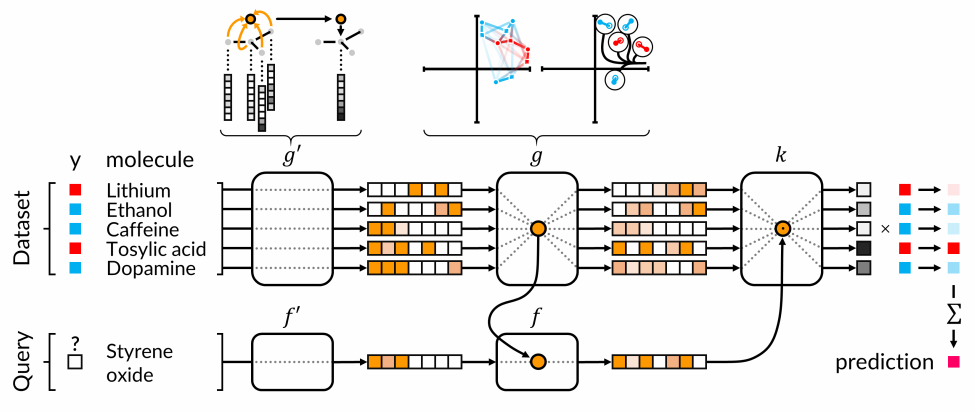
\includegraphics{Images/For_Table_Of_Contents_Only.png}
\end{figure}

Synopsis: We demonstrate how one-shot learning can lower the amount of data required to make meaningful predictions in drug discovery. Our architecture, the iterative refinement LSTM, permits the learning of meaningful distance metrics on small-molecule space.


\subsection{Definitions of Graph Primitives}

There are three major neural-network layers that are used to featurizing the molecular graphs. This is the graph convolution, $h_{\rm conv}(G)$, the graph pool, $h_{\rm pool}(G)$, and the graph gather, $h_{\rm gather}(G)$, all defined below. The graph convolution and graph pool operations definitions are given for a single node in the graph $v\in V$; however, when performing the operation on the graph, $G$, the operation is performed on all nodes simultaneously. This means that $h_{\rm conv}(G) = [h_{\rm conv}(v_1), h_{\rm conv}(v_2),\dots]$, and similarly for the pool layer. Specifically, we define
%\begin{equation*}
%\mathbf{h}_i^\prime, \mathbf{c}_i^\prime = 
%\begin{cases}
%{\rm{LSTM0}}\left(\mathbf{u}_i,\mathbf{h}_i,\mathbf{c}_i\right) &\mbox{if } %\mathbf{y}_i=0\\
%{\rm{LSTM1}}\left(\mathbf{u}_i,\mathbf{h}_i,\mathbf{c}_i\right) &\mbox{if } \mathbf{y}_i=1
%\end{cases}
%\end{equation*}
%Then 
%\begin{equation*}
%\mathbf{h}^\prime,\mathbf{c}^\prime = %{\rm{LSTM}}\left(\mathbf{u},\mathbf{h},\mathbf{c}\mid \mathbf{y}\right)
%\end{equation*}
\begin{align*}
h_{\rm{conv}}(v) &= \sigma\left(\sum\limits_{(u,v)\in E} W^{{\rm{deg}}(v)}v + U^{{\rm{deg}}(v)}u + b^{{\rm{deg}}(v)}\right) \\
h_{\rm{pool}}(v) &= \max\left\{\max\limits_{(u,v)\in E} u, v\right \} \\
h_{\rm{gather}}(G) &= \sum_{u\in V} u\\
\end{align*}
where $\sigma(\cdot)$ is a nonlinearity, such as ReLU or tanh.

\subsection{Convolutional Architecture in this Paper}

The Graph Conv, Siamese, AttnLSTM, and IterRefLSTM models all used the same convolutional architecture, shown in the table below, with the input starting at the left, sequentially feeding into the layers to the right.

We note that we did not make a focused effort at hyperparameter optimization in this work. Once we found the basic architecture below (by analogy with image convolutional networks), we proceeded with experimental evaluation. We leave thorough hyperparameter optimization to future work.

\begin{table}
    \begin{tabular}{ r | c | c | c | c | c | c | c | c |}
    \cline{2-9}
    layer & conv & pool & conv & pool & conv & pool & dense & gather\\
    dimension & 64 & & 128 & & 64 & & 128 &\\
    nonlinarity & relu & & relu & & relu & & tanh & tanh\\
    \cline{2-9}
    \end{tabular}
    
    \captionof{table}{Convolutional Network Architecture}
\end{table}

\subsection{Iterative Refinement LSTM Architecture in this paper}

The IterRefLSTM model and AttnLSTM model both use cosine similarity functions, $k(x,y) = \frac{x\cdot y}{ \left\|x\right\|\left\|y\right\|}$. All LSTMs used in this paper have an tanh activation, and hard sigmoid inner activation.

\subsection{Molecular Features}

For the convolutional models, all molecules were featurized into graphs by considering atoms as nodes and bonds as edges in an undirected graph. No distinction was made between bond types. RDKit \cite{landrum2016} was used to compute basic features of atoms including atom-type, valences, formal charges, and hybridization for each atom in a given molecule. This set  of features formed the initial set of atomic features fed into graph-convolutional layers. 

\subsection{Details of Model Training}
This section provides further information on model training procedures. All code for this paper is open-sourced, so we refer interested readers to the actual code within DeepChem for exact implementation details.
\paragraph{One-shot models}
When training a model on a dataset collection, assays within that collection are split into training assays and testing assays. For Tox21, 9 assays are reserved for training, 3 for testing. For SIDER, 21 assays are reserved for training, and 6 for testing. For MUV, 12 assays are reserved for training, and 5 models are reserved for testing. See following appendix sections for listings of training/testing assays for each collection.

As mentioned previously, training for one-shot models consists of a sequence of episodes. In each episode, an assay from the training assays is randomly sampled, then a support $S$ of size $n_\textrm{pos} + n_\textrm{neg}$ and a batch of queries $B$ (of size $128$) are sampled from the task. In the experimental tables, we use short-hand 10+/10- or 1+/5- to respectively represent $n_\textrm{pos} = 10, n_\textrm{neg}=10$ and $n_\textrm{pos}=1,n_\textrm{neg}=5$. Models were trained for $2000\cdot n_\textrm{train}$ episodes, where $n_\textrm{train}$ was the number of training assays for that dataset collection. Each episode takes one gradient descent step minimizing $\mathcal{L}$, using ADAM \cite{kingma2014adam}.

At test time, the accuracy of a one-shot model is evaluated separately on each testing assay. For a given test assay, a support of size $n_\textrm{pos} + n_\textrm{neg}$ is sampled at random from datapoints for that assay. The ROC-AUC score for the one-shot model is evaluated on the remainder of the datapoints for the test assay (excluding the support). This procedure is reported $20$ times for each test assay, and the mean and standard deviations of computed ROC-AUC scores for each test assay are presented in the tables in the appendix. For the tables in the body of the paper, the mean and standard deviations of computed ROC-AUC scores is only presented for the ``median task''. That is, for the test assay whose mean ROC-AUC score (over sampled supports) is the median of the set of mean ROC-AUC scores (over all test assays).

\paragraph{Singletask models}
Random forests were trained on circular fingerprint representations of input molecules \cite{rogers2010extended}. For each test assay, supports of size $n_\textrm{pos} + n_\textrm{neg}$ are sampled at random. The random forest model is trained on this sampled supported set, and evaluated on the remainder of test assay. This procedure is repeated $20$ times (note that a different random forest is trained for each newly sampled support). Means and standard deviations are reported as for one-shot models.

Singletask graph convolutional networks are trained as the random forests are, but with graph convolutional features instead of circular fingerprint representations.

\subsection{Tox21 Details}

\paragraph{Assay Details}
The assays NR-AR, NR-AR-LBD, NR-AhR, NR-Aromatase, NR-ER, NR-ER-LBD, NR-PPAR-gamma, SR-ARE, SR-ATAD5 were used for training. Assays SR-HSE, SR-MMP, and SR-p53 were used for model evaluation.

\paragraph{Per-Assay Results}
Results for each held-out assay are reported in Tables~\ref{tab:tox21-sr-hse},~\ref{tab:tox21-sr-mmp},~\ref{tab:tox21-sr-p53}.
\begin{table}[h]
    \centering
    \begin{tabular}{ |c|c|c|c|c|c| } 
    \hline
    SR-HSE & RF (100 trees) & Graph Conv & Siamese & AttnLSTM & IterRefLSTM \\ 
    \hline
    10+/10- & $0.532 \pm 0.033$& $0.540 \pm 0.025$ & $0.767 \pm 0.005$ & $0.747 \pm 0.003$ & $\mathbf{0.772 \pm 0.002}$ \\
    \hline
    5+/10- & $0.521 \pm 0.037$ & $0.546 \pm 0.023$ & $0.733 \pm 0.098$ & $0.716 \pm 0.098$ & $\mathbf{0.771 \pm 0.002}$ \\ 
    \hline
    1+/10- & $0.525 \pm 0.033$ & $0.531 \pm 0.035$ & $0.647 \pm 0.202$ & $0.498 \pm 0.046$ & $\mathbf{0.671 \pm 0.007}$ \\ 
    \hline
    1+/5- & $0.510 \pm 0.041$ & $0.537 \pm 0.043$ & $0.680 \pm 0.167$ & $0.505 \pm 0.074$ & $\mathbf{0.729 \pm 0.003}$ \\ 
    \hline
    1+/1- & $0.507 \pm 0.039$ & $0.526 \pm 0.0378$ & $0.613 \pm 0.187$ & $0.507 \pm 0.029$ & $\mathbf{0.767 \pm 0.001}$\\ 
    \hline
    \end{tabular}
    \caption{ROC-AUC scores of models on Tox21 assay SR-HSE. Numbers reported are means and standard deviations. Each model is evaluated 20 times with different support sets to compute means and standard deviations. The model with highest mean in each row is highlighted. The notation 10+/10- indicates supports with $10$ positive examples and $10$ negative examples.}
    \label{tab:tox21-sr-hse}
\end{table}
\begin{table}[h]
    \centering
    \begin{tabular}{ |c|c|c|c|c|c| } 
    \hline
    SR-MMP & RF (100 trees) & Graph Conv & Siamese & AttnLSTM & IterRefLSTM \\ 
    \hline
    10+/10- & $0.629 \pm 0.058$ & $0.648 \pm 0.029$ & $0.825 \pm 0.006$ & $0.801 \pm 0.001$ & $\mathbf{0.838 \pm 0.001}$ \\
    \hline
    5+/10- & $0.634 \pm 0.079$ & $0.637 \pm 0.061$ & $0.846 \pm 0.028$ & $0.811 \pm 0.003$ & $\mathbf{0.847 \pm 0.001}$ \\ 
    \hline
    1+/10- & $0.587 \pm 0.068$ & $0.541 \pm 0.093$ & $\mathbf{0.809 \pm 0.020}$ & $0.551 \pm 0.086$ & $0.730 \pm 0.003$ \\ 
    \hline
    1+/5- & $0.597 \pm 0.097$ & $0.595 \pm 0.086$ & $0.687 \pm 0.210$ & $0.602 \pm 0.122$ & $\mathbf{0.799 \pm 0.002}$ \\ 
    \hline
    1+/1- & $0.560 \pm 0.0844$ & $0.589 \pm 0.068$ & $0.657 \pm 0.222$ & $0.527 \pm 0.090$ & $\mathbf{0.835 \pm 0.001}$\\ 
    \hline
    \end{tabular}
    \caption{ROC-AUC scores of models on Tox21 assay SR-MMP. Numbers reported are means and standard deviations. Each model is evaluated 20 times with different support sets to compute means and standard deviations. The model with highest mean in each row is highlighted. The notation 10+/10- indicates supports with $10$ positive examples and $10$ negative examples.}
    \label{tab:tox21-sr-mmp}
\end{table}
\begin{table}[h]
    \centering
    \begin{tabular}{ |c|c|c|c|c|c| } 
    \hline
    SR-p53 & RF (100 trees) & Graph Conv & Siamese & AttnLSTM & IterRefLSTM \\ 
    \hline
    10+/10- & $0.586 \pm 0.056$ & $0.653 \pm 0.021$ & $0.820 \pm 0.003$ & $0.809 \pm 0.002$ & $\mathbf{0.823 \pm 0.002}$ \\
    \hline
    5+/10- & $0.573 \pm 0.0604$ & $0.639 \pm 0.042$ & $0.823 \pm 0.004$ & $0.753 \pm 0.173$ & $\mathbf{0.830 \pm 0.001}$ \\ 
    \hline
    1+/10- & $0.551 \pm 0.067$ & $0.597 \pm 0.083$ & $\mathbf{0.726 \pm 0.173}$ & $0.549 \pm 0.088$ & $0.724 \pm 0.008$ \\ 
    \hline
    1+/5- & $0.559 \pm 0.063$ & $0.595 \pm 0.073$ & $0.745 \pm 0.156$ & $0.593 \pm 0.153$ & $\mathbf{0.795 \pm 0.005}$ \\ 
    \hline
    1+/1- & $0.535 \pm 0.056$ & $0.591 \pm 0.084$ & $0.680 \pm 0.197$ & $0.507 \pm 0.079$ & $\mathbf{0.827 \pm 0.001}$\\ 
    \hline
    \end{tabular}
    \caption{ROC-AUC scores of models on Tox21 assay SR-p53. Numbers reported are means and standard deviations. Each model is evaluated 20 times with different support sets to compute means and standard deviations. The model with highest mean in each row is highlighted. The notation 10+/10- indicates supports with $10$ positive examples and $10$ negative examples.}
    \label{tab:tox21-sr-p53}
\end{table}

\subsection{SIDER Details}
\paragraph{Assay Details}
Indications "Hepatobiliary disorders", "Metabolism and nutrition disorders", "Product issues", "Eye disorders", "Investigations,Musculoskeletal and connective tissue disorders", "Gastrointestinal disorders", "Social circumstances", "Immune system disorders", "Reproductive system and breast disorders", "Neoplasms benign, malignant and unspecified (incl cysts and polyps)", "General disorders and administration site conditions", "Endocrine disorders", "Surgical and medical procedures", "Vascular disorders", "Blood and lymphatic system disorders", "Skin and subcutaneous tissue disorders", "Congenital, familial and genetic disorders", "Infections and infestations","Respiratory, thoracic and mediastinal disorders", "Psychiatric disorders" were used for training. Indications "Renal and urinary disorders", "Pregnancy, puerperium and perinatal conditions", "Ear and labyrinth disorders", "Cardiac disorders", "Nervous system disorders", "Injury, poisoning and procedural complications" were used for model evaluation.

\paragraph{Per-Assay Results}
Results for each held-out assay in SIDER collection are reported in Tables~\ref{tab:sider-rud}, ~\ref{tab:sider-pppc}, ~\ref{tab:sider-eld}, ~\ref{tab:sider-cd}, ~\ref{tab:sider-nsd}, ~\ref{tab:sider-ispc}.
\begin{table}[h]
    \centering
    \begin{tabular}{ |c|c|c|c|c|c| } 
    \hline
    R.U.D & RF (100 trees) & Graph Conv & Siamese & AttnLSTM & IterRefLSTM \\ 
    \hline
    10+/10- & $0.564 \pm 0.031$ & $0.496 \pm 0.035$ & $\mathbf{0.729 \pm 0.049}$ & $0.576 \pm 0.081$ & $0.706 \pm 0.002$ \\
    \hline
    5+/10- & $0.564 \pm 0.022$ & $0.477 \pm 0.031$ & $0.670 \pm 0.119$ & $0.540 \pm 0.026$ & $\mathbf{0.710 \pm 0.002}$ \\ 
    \hline
    1+/10- & $0.540 \pm 0.034$ & $0.449 \pm 0.025$ & $\mathbf{0.578 \pm 0.047}$ & $0.518 \pm 0.025$ & $0.575 \pm 0.015$ \\ 
    \hline
    1+/5- & $0.538 \pm 0.045$ & $0.457 \pm 0.029$ & $0.518 \pm 0.060$ & $0.509 \pm 0.026$ & $\mathbf{0.681 \pm 0.010}$ \\ 
    \hline
    1+/1- & $0.508 \pm 0.046$ & $0.468 \pm 0.045$ & $0.503 \pm 0.063$ & $0.497 \pm 0.022$ & $\mathbf{0.728 \pm 0.001}$\\ 
    \hline
    \end{tabular}
    \caption{ROC-AUC scores of models on "Renal and urinary disorders". Numbers reported are means and standard deviations. Each model is evaluated 20 times with different support sets to compute means and standard deviations. The model with highest mean in each row is highlighted. The notation 10+/10- indicates supports with $10$ positive examples and $10$ negative examples.}
    \label{tab:sider-rud}
\end{table}
\begin{table}[h]
    \centering
    \begin{tabular}{ |c|c|c|c|c|c| } 
    \hline
    P.P.P.C & RF (100 trees) & Graph Conv & Siamese & AttnLSTM & IterRefLSTM \\ 
    \hline
    10+/10- & $0.515 \pm 0.034$ & $0.552 \pm 0.028$ & $\mathbf{0.694 \pm 0.012}$ & $0.505 \pm 0.018$ & $0.669 \pm 0.007$ \\
    \hline
    5+/10- & $0.517 \pm 0.050$ & $0.548 \pm 0.032$ & $0.645 \pm 0.073$ & $0.545 \pm 0.041$ & $\mathbf{0.714 \pm 0.004}$ \\ 
    \hline
    1+/10- & $0.529 \pm 0.043$ & $0.521 \pm 0.041$ & $\mathbf{0.541 \pm 0.038}$ & $0.505 \pm 0.026$ & $0.539 \pm 0.018$ \\ 
    \hline
    1+/5- & $0.507 \pm 0.044$ & $0.538 \pm 0.030$ & $0.511 \pm 0.032$ & $0.505 \pm 0.022$ & $\mathbf{0.640 \pm 0.011}$ \\ 
    \hline
    1+/1- & $0.504 \pm 0.032$ & $0.527 \pm 0.027$ & $0.510 \pm 0.016$ & $0.493 \pm 0.016$ & $\mathbf{0.697 \pm 0.002}$\\ 
    \hline
    \end{tabular}
    \caption{ROC-AUC scores of models on ``Pregnancy, puerperium and perinatal conditions''. Numbers reported are means and standard deviations. Each model is evaluated 20 times with different support sets to compute means and standard deviations. The model with highest mean in each row is highlighted. The notation 10+/10- indicates supports with $10$ positive examples and $10$ negative examples.}
    \label{tab:sider-pppc}
\end{table}
\begin{table}[h]
    \centering
    \begin{tabular}{ |c|c|c|c|c|c| } 
    \hline
    E.L.D & RF (100 trees) & Graph Conv & Siamese & AttnLSTM & IterRefLSTM \\ 
    \hline
    10+/10- & $0.527 \pm 0.034$ & $0.533 \pm 0.026$ & $\mathbf{0.676 \pm 0.077}$ & $0.559 \pm 0.070$ & $0.661 \pm 0.001$ \\
    \hline
    5+/10- & $0.518 \pm 0.038$ & $0.486 \pm 0.032$ & $0.648 \pm 0.070$ & $0.528 \pm 0.047$ & $\mathbf{0.680 \pm 0.001}$ \\ 
    \hline
    1+/10- & $0.524 \pm 0.021$ & $0.456 \pm 0.018$ & $0.547 \pm 0.037$ & $0.506 \pm 0.016$ & $\mathbf{0.558 \pm 0.011}$ \\ 
    \hline
    1+/5- & $0.526 \pm  0.031$ & $0.463 \pm 0.027$ & $0.534 \pm 0.064$ & $0.504 \pm 0.021$ & $\mathbf{0.639 \pm 0.008}$ \\ 
    \hline
    1+/1- & $0.509 \pm 0.032$ & $0.519 \pm 0.035$ & $0.514 \pm 0.059$ & $0.501 \pm 0.022$ & $\mathbf{0.689 \pm 0.001}$\\ 
    \hline
    \end{tabular}
    \caption{ROC-AUC scores of models on ``Ear and labyrinth disorders''. Numbers reported are means and standard deviations. Each model is evaluated 20 times with different support sets to compute means and standard deviations. The model with highest mean in each row is highlighted. The notation 10+/10- indicates supports with $10$ positive examples and $10$ negative examples.}
    \label{tab:sider-eld}
\end{table}
\begin{table}[h]
    \centering
    \begin{tabular}{ |c|c|c|c|c|c| } 
    \hline
    C.D & RF (100 trees) & Graph Conv & Siamese & AttnLSTM & IterRefLSTM \\ 
    \hline
    10+/10- & $0.552 \pm 0.036$ & $0.456 \pm 0.038$ & $0.687 \pm 0.089$ & $0.532 \pm 0.076$ & $\mathbf{0.691 \pm 0.002}$ \\
    \hline
    5+/10- & $0.560 \pm 0.041$ & $0.444 \pm 0.027$ & $0.678 \pm 0.085$ & $0.534 \pm 0.053$ & $\mathbf{0.704 \pm 0.002}$ \\ 
    \hline
    1+/10- & $0.540 \pm 0.029$ & $0.422 \pm 0.035$ & $0.544 \pm 0.056$ & $0.504 \pm 0.016$ & $\mathbf{0.555 \pm 0.012}$ \\ 
    \hline
    1+/5- & $0.537 \pm 0.052$ & $0.447 \pm 0.035$ & $0.536 \pm 0.052$ & $0.517 \pm 0.045$ & $\mathbf{0.674 \pm 0.005}$ \\ 
    \hline
    1+/1- & $0.506 \pm 0.039$ & $0.461 \pm 0.0478$ & $0.543 \pm 0.068$ & $0.509 \pm 0.029$ & $\mathbf{0.704 \pm 0.001}$\\ 
    \hline
    \end{tabular}
    \caption{ROC-AUC scores of models on ``Cardiac disorders''. Numbers reported are means and standard deviations. Each model is evaluated 20 times with different support sets to compute means and standard deviations. The model with highest mean in each row is highlighted. The notation 10+/10- indicates supports with $10$ positive examples and $10$ negative examples.}
    \label{tab:sider-cd}
\end{table}
\begin{table}[h]
    \centering
    \begin{tabular}{ |c|c|c|c|c|c| } 
    \hline
    N.S.D & RF (100 trees) & Graph Conv & Siamese & AttnLSTM & IterRefLSTM \\ 
    \hline
    10+/10- & $0.681 \pm 0.077$ & $0.367 \pm 0.040$ & $0.809 \pm 0.013$ & $0.657 \pm 0.119$ & $\mathbf{0.784 \pm 0.006}$ \\
    \hline
    5+/10- & $0.638 \pm 0.102$ & $0.360 \pm 0.035$ & $0.791 \pm 0.022$ & $0.637 \pm 0.078$ & $\mathbf{0.803 \pm 0.007}$ \\ 
    \hline
    1+/10- & $0.639 \pm 0.043$ & $0.334 \pm 0.025$ & $0.631 \pm 0.115$ & $0.511 \pm 0.057$ & $\mathbf{0.667 \pm 0.021}$ \\ 
    \hline
    1+/5- & $0.604 \pm 0.091$ & $0.344 \pm 0.033$ & $0.617 \pm 0.107$ & $0.514 \pm 0.080$ & $\mathbf{0.775 \pm 0.011}$ \\ 
    \hline
    1+/1- & $0.598 \pm 0.100$ & $0.437 \pm 0.095$ & $0.515 \pm 0.121$ & $0.508 \pm 0.060$ & $\mathbf{0.797 \pm 0.002}$\\ 
    \hline
    \end{tabular}
    \caption{ROC-AUC scores of models on ``Nervous system disorders''. Numbers reported are means and standard deviations. Each model is evaluated 20 times with different support sets to compute means and standard deviations. The model with highest mean in each row is highlighted. The notation 10+/10- indicates supports with $10$ positive examples and $10$ negative examples.}
    \label{tab:sider-nsd}
\end{table}
\begin{table}[h]
    \centering
    \begin{tabular}{ |c|c|c|c|c|c| } 
    \hline
    I.S.P.C & RF (100 trees) & Graph Conv & Siamese & AttnLSTM & IterRefLSTM \\ 
    \hline
    10+/10- & $0.535 \pm 0.036$ & $0.483 \pm 0.026$ & $\mathbf{0.671 \pm 0.089}$ & $0.553 \pm 0.058$ & $0.667 \pm 0.001$ \\
    \hline
    5+/10- & $0.533 \pm 0.0302$ & $0.473 \pm 0.029$ & $0.589 \pm 0.125$ & $0.509 \pm 0.036$ & $\mathbf{0.688 \pm 0.002}$ \\ 
    \hline
    1+/10- & $0.541 \pm 0.021$ & $0.447 \pm 0.016$ & $0.537 \pm 0.045$ & $0.510 \pm 0.015$ & $\mathbf{0.556 \pm 0.011}$ \\ 
    \hline
    1+/5- & $0.529 \pm 0.028$ & $0.458 \pm 0.024$ & $0.530 \pm 0.050$ & $0.501 \pm 0.021$ & $\mathbf{0.644 \pm 0.012}$ \\ 
    \hline
    1+/1- & $0.477 \pm 0.029$ & $0.475 \pm 0.023$ & $0.501 \pm 0.044$ & $0.504 \pm 0.019$ & $\mathbf{0.689 \pm 0.001}$\\ 
    \hline
    \end{tabular}
    \caption{ROC-AUC scores of models on ``Injury, poisoning and procedural complications''. Numbers reported are means and standard deviations. Each model is evaluated 20 times with different support sets to compute means and standard deviations. The model with highest mean in each row is highlighted. The notation 10+/10- indicates supports with $10$ positive examples and $10$ negative examples.}
    \label{tab:sider-ispc}
\end{table}

\subsection{MUV Details}
\paragraph{Assay Details}
Assays MUV-466, MUV-548, MUV-600, MUV-644, MUV-652, MUV-689, MUV-692, MUV-712, MUV-713, MUV-733, MUV-737, MUV-810 were used for training. Assays MUV-832, MUV-846, MUV-852,  MUV-858, MUV-859 were used for model evaluation.
\paragraph{Per-Assay Results}
Results for each held-out assay in MUV collection are reported in Tables ~\ref{tab:muv-832}, ~\ref{tab:muv-846}, ~\ref{tab:muv-852}, ~\ref{tab:muv-858}, ~\ref{tab:muv-859}.
\begin{table}[h]
    \centering
    \begin{tabular}{ |c|c|c|c|c|c| } 
    \hline
    MUV-832 & RF (100 trees) & Graph Conv & Siamese & AttnLSTM & IterRefLSTM \\ 
    \hline
    10+/10- & $\mathbf{0.805 \pm 0.0547}$ & $0.568 \pm 0.0851$ & $0.655 \pm 0.066$ & $0.484 \pm 0.058$ & $0.500 \pm 0.053$ \\
    \hline
    5+/10- & $\mathbf{0.730 \pm 0.063}$ & $0.565 \pm 0.068$ & $0.656 \pm 0.136$ & $0.517 \pm 0.045$ & $0.726 \pm 0.025$ \\ 
    \hline
    1+/10- & $0.556 \pm 0.084$ & $0.569 \pm 0.061$ & $\mathbf{0.610 \pm 0.144}$ & $0.511 \pm 0.042$ & $0.573 \pm 0.013$ \\ 
    \hline
    1+/5- & $0.598 \pm 0.067$ & $0.573 \pm 0.082$ & $0.511 \pm 0.179$ & $0.529 \pm 0.052$ & $\mathbf{0.670 \pm 0.014}$ \\ 
    \hline
    1+/1- & $\mathbf{0.559 \pm 0.095}$ & $0.552 \pm 0.084$ & $0.500 \pm 0.001$ & $0.497 \pm 0.030$ & $0.463 \pm 0.024$\\ 
    \hline
    \end{tabular}
    \caption{ROC-AUC scores of models on MUV-832. Numbers reported are means and standard deviations. Each model is evaluated 20 times with different support sets to compute means and standard deviations. The model with highest mean in each row is highlighted. The notation 10+/10- indicates supports with $10$ positive examples and $10$ negative examples.}
    \label{tab:muv-832}
\end{table}
\begin{table}[h]
    \centering
    \begin{tabular}{ |c|c|c|c|c|c| } 
    \hline
    MUV-846 & RF (100 trees) & Graph Conv & Siamese & AttnLSTM & IterRefLSTM \\ 
    \hline
    10+/10- & $\mathbf{0.820 \pm 0.051}$ & $0.608 \pm 0.079$ & $0.601 \pm 0.041$ & $0.504 \pm 0.058$ & $0.460 \pm 0.054$ \\
    \hline
    5+/10- & $\mathbf{0.788 \pm 0.061}$ & $0.595 \pm 0.063$ & $0.655 \pm 0.166$ & $0.494 \pm 0.040$ & $0.663 \pm 0.019$ \\ 
    \hline
    1+/10- & $\mathbf{0.700 \pm 0.094}$ & $0.576 \pm 0.075$ & $0.602 \pm 0.118$ & $0.504 \pm 0.045$ & $0.598 \pm 0.013$ \\ 
    \hline
    1+/5- & $\mathbf{0.698 \pm 0.106}$ & $0.554 \pm 0.089$ & $ 0.562 \pm 0.149$ & $0.517 \pm 0.059$ & $0.632 \pm 0.011$ \\ 
    \hline
    1+/1- & $\mathbf{0.646 \pm 0.080}$ & $0.588 \pm 0.077$ & $0.500 \pm 0.0001$ & $0.496 \pm 0.015$ & $0.511 \pm 0.029$\\ 
    \hline
    \end{tabular}
    \caption{ROC-AUC scores of models on MUV-846. Numbers reported are means and standard deviations. Each model is evaluated 20 times with different support sets to compute means and standard deviations. The model with highest mean in each row is highlighted. The notation 10+/10- indicates supports with $10$ positive examples and $10$ negative examples.}
    \label{tab:muv-846}
\end{table}
\begin{table}[h]
    \centering
    \begin{tabular}{ |c|c|c|c|c|c| } 
    \hline
    MUV-852 & RF (100 trees) & Graph Conv & Siamese & AttnLSTM & IterRefLSTM \\ 
    \hline
    10+/10- & $\mathbf{0.754 \pm 0.064}$ & $0.657 \pm 0.103$ & $0.678 \pm 0.047$ & $0.514 \pm 0.049$ & $0.514 \pm 0.048$ \\
    \hline
    5+/10- & $\mathbf{0.775 \pm 0.047}$ & $0.670 \pm 0.068$ & $0.765 \pm 0.017$ & $0.495 \pm 0.046$ & $0.755 \pm 0.023$ \\ 
    \hline
    1+/10- & $0.631 \pm 0.105$ & $0.627 \pm 0.156$ & $\mathbf{0.737 \pm 0.097}$ & $0.574 \pm 0.053$ & $0.569 \pm 0.012$ \\ 
    \hline
    1+/5- & $0.632 \pm 0.106$ & $0.597 \pm 0.135$ & $0.663 \pm 0.109$ & $0.485 \pm 0.022$ & $\mathbf{0.727 \pm 0.008}$ \\ 
    \hline
    1+/1- & $0.590 \pm 0.134$ & $\mathbf{0.614 \pm 0.133}$ & $0.500 \pm 0.002$ & $0.502 \pm 0.032$ & $0.471 \pm 0.032$ \\ 
    \hline
    \end{tabular}
    \caption{ROC-AUC scores of models on MUV-852. Numbers reported are means and standard deviations. Each model is evaluated 20 times with different support sets to compute means and standard deviations. The model with highest mean in each row is highlighted. The notation 10+/10- indicates supports with $10$ positive examples and $10$ negative examples.}
    \label{tab:muv-852}
\end{table}
\begin{table}[h]
    \centering
    \begin{tabular}{ |c|c|c|c|c|c| } 
    \hline
    MUV-858 & RF (100 trees) & Graph Conv & Siamese & AttnLSTM & IterRefLSTM \\ 
    \hline
    10+/10- & $\mathbf{0.565 \pm 0.073}$ & $0.552 \pm 0.083$ & $0.550 \pm 0.143$ & $0.516 \pm 0.053$ & $0.530 \pm 0.044$ \\
    \hline
    5+/10- & $0.564 \pm 0.072$ & $0.554 \pm 0.069$ & $0.580 \pm 0.105$ & $0.548 \pm 0.051$ & $\mathbf{0.629 \pm 0.023}$ \\ 
    \hline
    1+/10- & $0.537 \pm 0.089$ & $0.552 \pm 0.069$ & $0.553 \pm 0.101$ & $0.492 \pm 0.032$ & $\mathbf{0.567 \pm 0.014}$ \\ 
    \hline
    1+/5- & $0.577 \pm 0.068$ & $0.526 \pm 0.050$ & $0.486 \pm 0.082$ & $0.506 \pm 0.028$ & $\mathbf{0.613 \pm 0.009}$ \\ 
    \hline
    1+/1- & $\mathbf{0.526 \pm 0.070}$ & $\mathbf{0.527 \pm 0.060}$ & $0.500 \pm 0.009$ & $0.500 \pm 0.027$ & $0.503 \pm 0.041$ \\ 
    \hline
    \end{tabular}
    \caption{ROC-AUC scores of models on MUV-858. Numbers reported are means and standard deviations. Each model is evaluated 20 times with different support sets to compute means and standard deviations. The model with highest mean in each row is highlighted. The notation 10+/10- indicates supports with $10$ positive examples and $10$ negative examples.}
    \label{tab:muv-858}
\end{table}

\begin{table}[h]
    \centering
    \begin{tabular}{ |c|c|c|c|c|c| } 
    \hline
    MUV-859 & RF (100 trees) & Graph Conv & Siamese & AttnLSTM & IterRefLSTM \\ 
    \hline
    10+/10- & $0.503 \pm 0.0717$ & $0.534 \pm 0.084$ & $0.514 \pm 0.054$ & $0.498 \pm 0.098$ & $0.474 \pm 0.059$ \\
    \hline
    5+/10- & $0.502 \pm 0.068$ & $0.510 \pm 0.067$ & $0.498 \pm 0.051$ & $0.507 \pm 0.052$ & $0.386 \pm 0.017$ \\ 
    \hline
    1+/10- & $0.530 \pm 0.053$ & $0.511 \pm 0.049$ & $0.507 \pm 0.062$ & $0.497 \pm 0.076$ & $0.412 \pm  0.010$ \\ 
    \hline
    1+/5- & $0.515 \pm 0.074$ & $0.513 \pm 0.042$ & $0.514 \pm 0.053$ & $0.515 \pm 0.021$ & $0.397 \pm 0.010$ \\ 
    \hline
    1+/1- & $0.521 \pm 0.060$ & $0.493 \pm 0.065$ & $0.500 \pm 0.001$ & $0.502 \pm 0.044$ & $0.479 \pm 0.037$ \\ 
    \hline
    \end{tabular}
    \caption{ROC-AUC scores of models on MUV-859. Numbers reported are means and standard deviations. Each model is evaluated 20 times with different support sets to compute means and standard deviations. No models had signal so did not highlight any models. The notation 10+/10- indicates supports with $10$ positive examples and $10$ negative examples.}
    \label{tab:muv-859}
\end{table}